\hypertarget{numerical-algorithms}{%
\section{Numerical Algorithms}\label{numerical-algorithms}}

\hypertarget{dense-matrix-vector-multiplication}{%
\subsection{Dense Matrix-Vector
Multiplication}\label{dense-matrix-vector-multiplication}}

\begin{itemize}
\tightlist
\item let $A$ be a $n*n$ matrix and $x$ and $y$ are $n*1$ vectors.
\item compute $y: Ax = y$
\end{itemize}

\hypertarget{row-wise-1d-partitioning-1-row-of-matrix-a-per-process}{%
\subsubsection{Row-wise 1D Partitioning: 1 row of matrix A per
process}\label{row-wise-1d-partitioning-1-row-of-matrix-a-per-process}}

\begin{figure}[H]
\centering
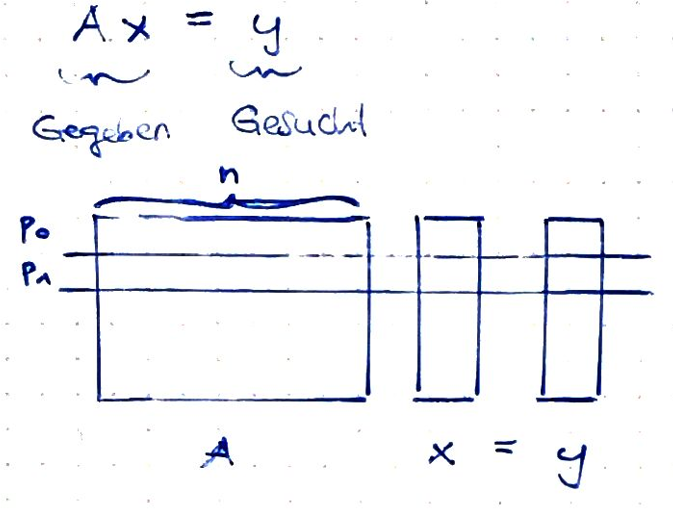
\includegraphics[width=0.4\textwidth]{figures/matrix-mult-partitioning.png}
\caption{Partitioning}
\end{figure}

\begin{figure}[H]
\centering
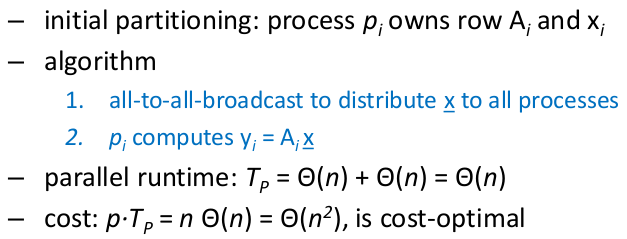
\includegraphics[width=0.5\textwidth]{figures/matrixVectorMulitplication1.png}
\caption{Vorgehen 1}
\end{figure}

\hypertarget{row-wise-1d-partitioning-using-fewer-than-n-processes}{%
\subsubsection{Row-wise 1D Partitioning: using fewer than n
processes}\label{row-wise-1d-partitioning-using-fewer-than-n-processes}}

\begin{figure}[H]
\centering
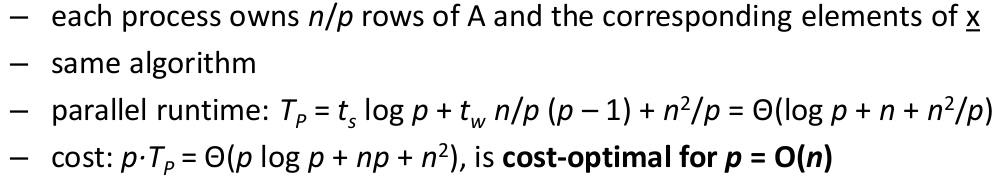
\includegraphics[width=0.8\textwidth]{figures/matrixVectorMulitplication2.png}
\caption{Vorgehen 2}
\end{figure}

\hypertarget{d-partitioning-1-matrix-element-per-process}{%
\subsubsection{2D Partitioning: 1 matrix element per
process}\label{d-partitioning-1-matrix-element-per-process}}

\begin{figure}[H]
\centering
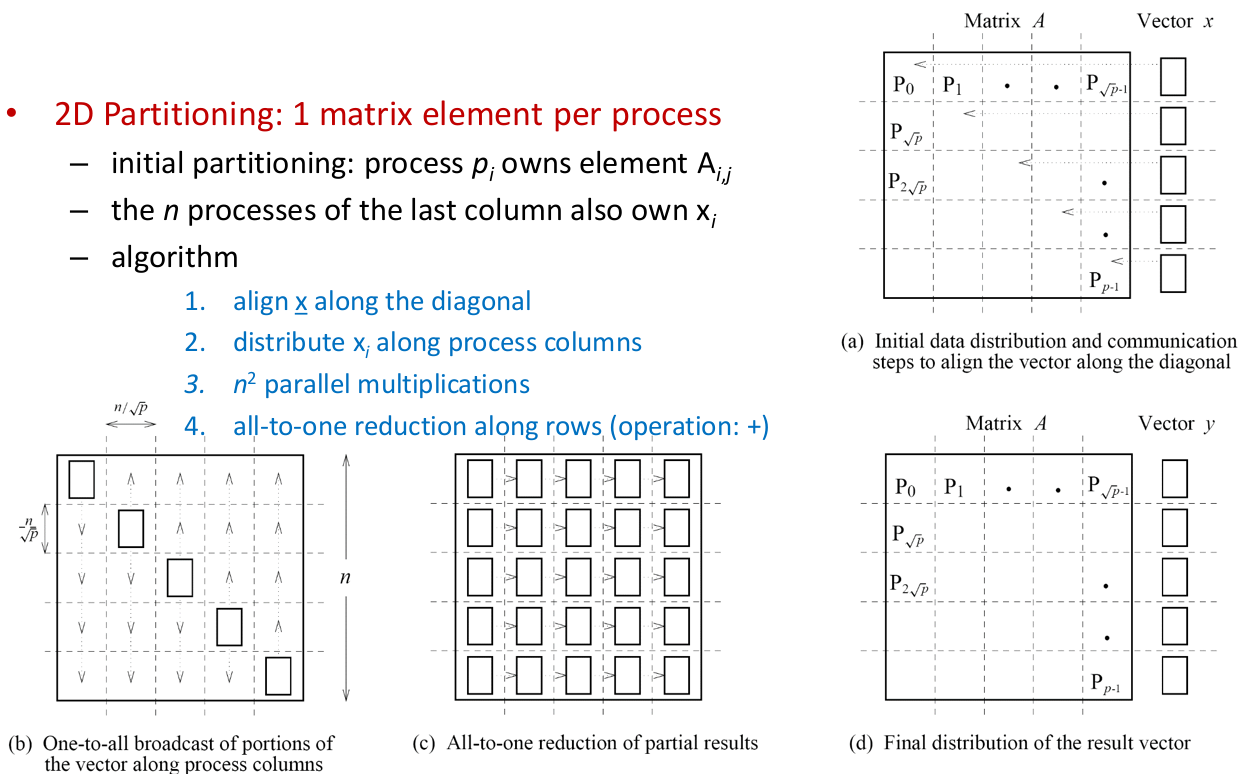
\includegraphics[width=1\textwidth]{figures/matrixVectorMulitplication3.png}
\caption{Vorgehen 3}
\end{figure}

\begin{enumerate}
\def\labelenumi{\arabic{enumi}.}
\tightlist
\item
  Jedes Matrix-Element gehört genau zu einem Prozess
\item
  Der Vector x wird an alle Prozesse verteilt, die auf der Diagnoale der
  Matrix liegen
\item
  Der Prozess X verteilt den erhaltenen Wert $X_i$ an die Prozesse in
  seiner Spalte
\item
  Ausführung der parallelen Multiplikationen
\item
  All-to-one Reduction in der eigenen Reihe
\end{enumerate}

\begin{figure}[H]
\centering
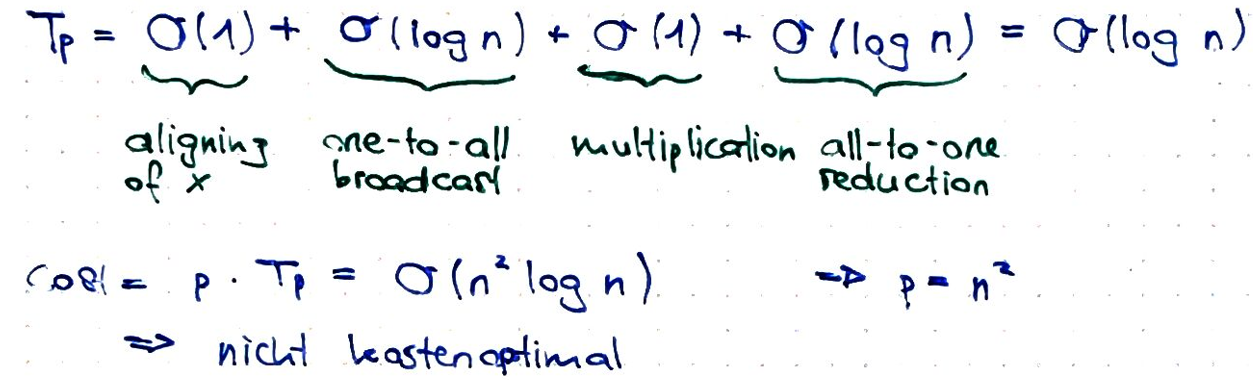
\includegraphics[width=0.7\textwidth]{figures/matrix-mult-2DPartitioning.png}
\caption{2D Partitioning}
\end{figure}
\clearpage

\hypertarget{d-partitioning-using-fewer-than-n-2-processes}{%
\subsubsection{2D Partitioning: using fewer than n 2
processes}\label{d-partitioning-using-fewer-than-n-2-processes}}

\begin{figure}[H]
\centering
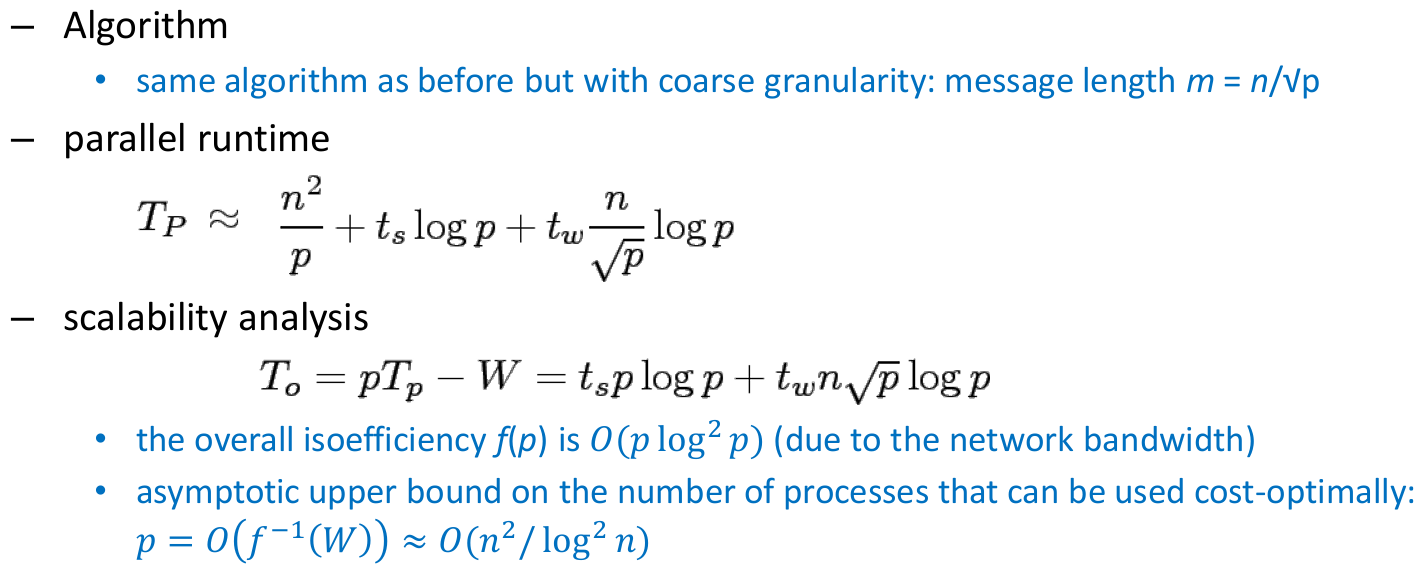
\includegraphics[width=0.9\textwidth]{figures/matrixVectorMulitplication4.png}
\caption{Vorgehen 4}
\end{figure}

\begin{figure}[H]
\centering
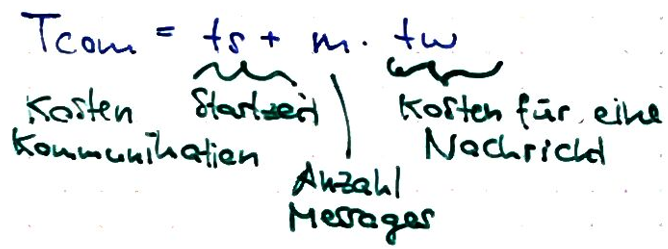
\includegraphics[width=0.5\textwidth]{figures/matrix-mult-comm-costs.png}
\caption{Communication Costs}
\end{figure}

\hypertarget{dense-matrix-matrix-multiplication}{%
\subsection{Dense Matrix-Matrix
Multiplication}\label{dense-matrix-matrix-multiplication}}

\begin{itemize}
\tightlist
\item
  let $A$ and $B$ be $n*n$ matrices
\item
  compute $C = A*B$
\end{itemize}

\hypertarget{matrix-multiplication-and-block-matrix-multiplication}{%
\subsubsection{Matrix Multiplication and Block Matrix
Multiplication}\label{matrix-multiplication-and-block-matrix-multiplication}}

$q$ determines granularity of block matrix multiplication $(1 < q \leq n)$.

\begin{figure}[H]
\centering
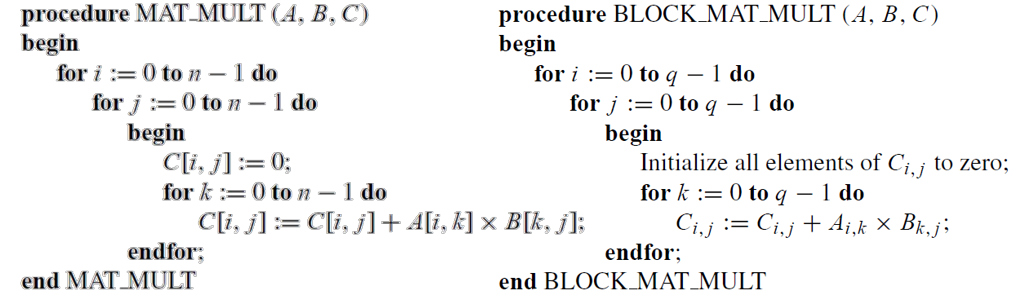
\includegraphics[width=0.9\textwidth]{figures/matrixMatrixMultiplication1.png}
\caption{Matrix Multiplication}
\end{figure}

\begin{figure}[H]
\centering
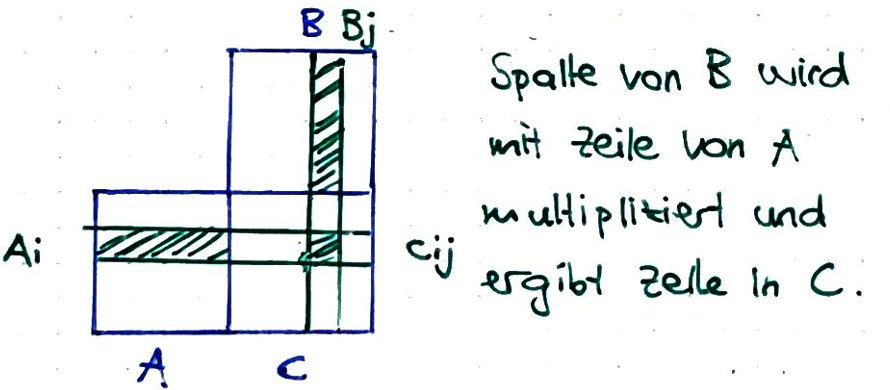
\includegraphics[width=0.5\textwidth]{figures/matrix-mult-block1}
\caption{Block-wise Matrix Multiplication 1}
\end{figure}

\begin{figure}[H]
\centering
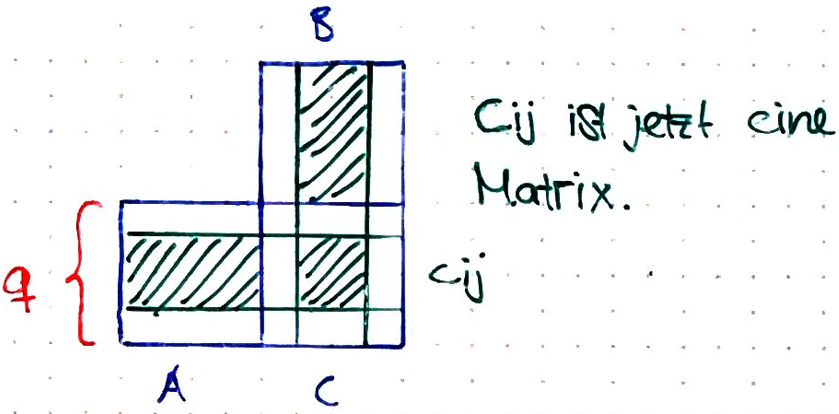
\includegraphics[width=0.5\textwidth]{figures/matrix-mult-block2}
\caption{Block-wise Matrix Multiplication 2}
\end{figure}

\hypertarget{a-simple-parallel-algorithm}{%
\subsubsection{A Simple Parallel
Algorithm}\label{a-simple-parallel-algorithm}}

\begin{figure}[H]
\centering
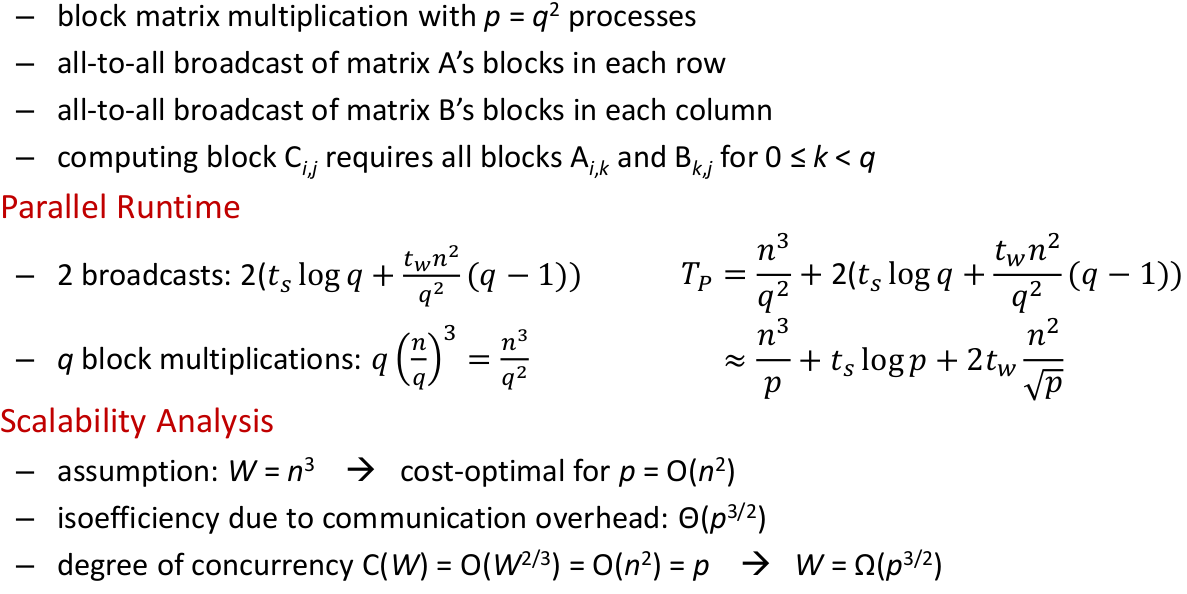
\includegraphics[width=0.9\textwidth]{figures/matrixMatrixMultiplication2.png}
\caption{Matrix Multiplication - Simple Algorithm}
\end{figure}

\hypertarget{cannons-matrix-multiplication}{%
\subsection{Cannon's Matrix
Multiplication}\label{cannons-matrix-multiplication}}

\begin{figure}[H]
\centering
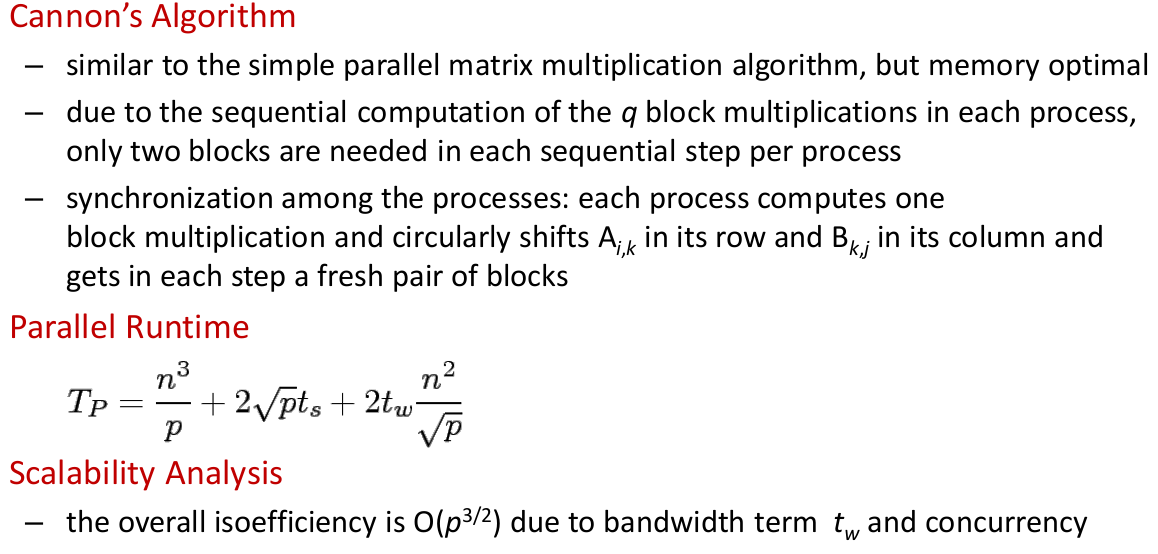
\includegraphics[width=0.8\textwidth]{figures/cannon.png}
\caption{Cannon's Matrix Multiplication}
\end{figure}

\begin{figure}[H]
\centering
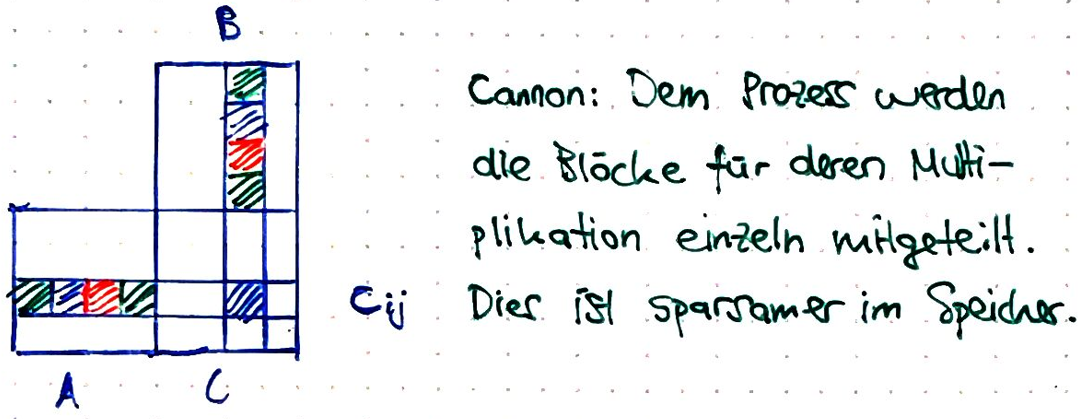
\includegraphics[width=0.7\textwidth]{figures/matrix-mult-cannon.png}
\caption{Principle of Cannon}
\end{figure}

\hypertarget{dna-matrix-multiplication}{%
\subsection{DNA Matrix Multiplication}\label{dna-matrix-multiplication}}

(Hier werden die Zwischendaten partitioniert)

\begin{figure}[H]
\centering
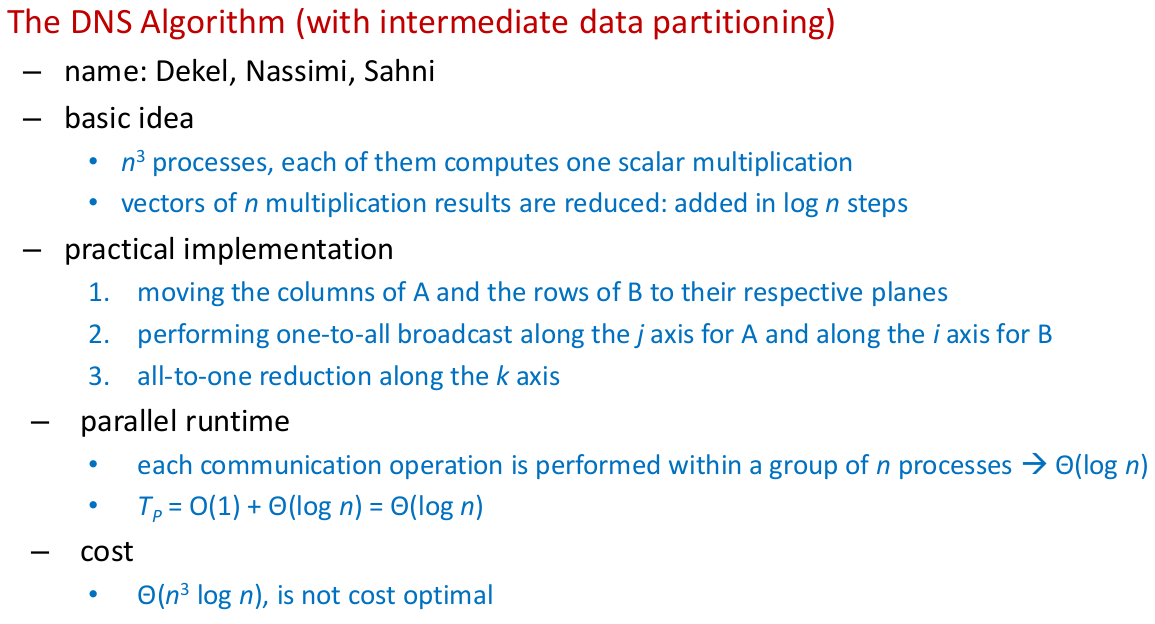
\includegraphics[width=0.8\textwidth]{figures/dnsMatrixMultiplication1.png}
\caption{DNS Matrix Multiplication}
\end{figure}

\clearpage